\section{Previous Implementations}
In this section we briefly describe the most used libraries at the moment that implement the Mapper algorithm. In particular, we focus on discussing their architecture and design choices, highlighting the corresponding pros and cons.


\subsection{Kepler Mapper}
\paragraph{Kepler Mapper}
Kepler Mapper is a pure Python implementation of the Mapper algorithm. It relies on clustering and filter functions implemented in the popular package Scikit-learn. However, compared to other implementations described further on, it is limited. It implements only one type of cover, and furthermore it does not compute the nerve of such cover, but only its one-dimensional skeleton. In other words, it completely ignores simplices with dimension $d, d>=1$. Such a one-dimensional skeleton is nothing else than a simple undirected graph.\\
As a filter function, the user can provide a Scikit-learn API compatible object (an object with a \lstinline|fit_transform()| method) or a user-made numpy.ndarray containing the filter values of the data points. As a clustering algorithm, Kepler Mapper uses Scikit-learn API compatible clustering algorithms, that means a class with the following methods: get\_params(), fit(), and the following attribute: \_labels.

At the present Kepler Mapper is under constant development ( as at the 10th of March 2019 the GitHub repo has 482 commits, 8 branches, 6 releases, last published commit the 6th of March 2019).

Kepler Mapper implements a very effective visualization of the output graph. The package provides a base HTML file, and uses Jinja2 to modify such a base HTML file with the data contained in the output graph to produce a new HTML file that renders the output graph.
\paragraph{Architecture}
This package (as in September 2018) is implemented in an OOP fashion, and consists of only three classes: KeplerMapper, Cover, GraphNerve. Figure \ref{fig:keplermapper} illustrates this simple architecture. This architecture is really simple if compared to the more complex one of Python Mapper (a second implementation of Mapper) illustrated in figure \ref{fig:pymapper}.
\paragraph{Example}
We present an easy use-case example of this package, discussing how the steps of Mapper were implemented in the package.
\begin{lstlisting}[language=Python, caption=Kepler Mapper example]
# Import the class
import kmapper as km

# Some sample data
from sklearn import datasets
data, labels = datasets.make_circles(n_samples=5000, noise=0.03, factor=0.3)

# Initialize
mapper = km.KeplerMapper(verbose=1)

# Fit to and transform the data
projected_data = mapper.project(data, projection=[0,1]) # X-Y axis

# Create dictionary called 'graph' with nodes, edges and meta-information
graph = mapper.map(projected_data, data, nr_cubes=10)

# Visualize it
mapper.visualize(graph, path_html="make_circles_keplermapper_output.html",
title="make_circles(n_samples=5000, noise=0.03, factor=0.3)")
\end{lstlisting}
\begin{itemize}
	\item Step 1: evaluating the filter function $f$. \\The filter values $f(X)$ are calculated in line 12. Internally, the KeplerMapper object uses functions imported from Numpy and Scikit-Learn to calculate the projection on the x-y axis of the data points. The user is just requested to insert as arguments of the $project()$ method a list of indices identifying the axis onto which to project the data.
	\item Step 2: computing the pullback cover $\mathcal B$. \\This step is done in line 15. The default cover implemented in Kepler Mapper is a uniform cover with 10 intervals and a percentage of overlap of 20\%. The user can modify this clustering algorithm by passing to the method $KeplerMapper.map()$ a Scikit-learn API compatible clusterer in the following way:
	\begin{lstlisting}[language=Python]
from kmapper.cover import Cover
graph = mapper.map(projected_data, data, nr_cubes=10, coverer=Cover(nintervals=15, perc_overlap=0.4))\end{lstlisting}
	\item Step 3: clustering the pre images $\{B_i\}$.\\This step is done again in line 15. The default clustering scheme implemented in Kepler Mapper is DBSCAN, implemented in $sklearn.cluster.DBSCAN()$. The user can modify this clustering algorithm by passing to the method KeplerMapper.map() a Scikit-learn API compatible clusterer in the following way:
	\begin{lstlisting}[language=Python]
custom_clusterer = sklearn.cluster.DBSCAN(eps=0.5, min_samples=3)
graph = mapper.map(projected_data, data, nr_cubes=10, clusterer=custom_clusterer)\end{lstlisting}
	\item Step 4: building the nerve complex. \\This step is done again in line 15 and the nerve complex is stored as a Python dictionary returned by the method $KeplerMapper.map()$. Such Python dictionary has the following keys: "nodes", "links", "simplices", and "metadata" where $graph["links"]$ and $graph["simplices"]$ are return values of a call to a GraphNerve functor.
	\item Step 5: visualizing the graph.\\Line 18. $KeplerMapper.visualize()$ is a really interesting method. In 35 lines of code it converts the information contained in the graph dictionary to a very effective HTML/D3.js visualization thanks to Jinja templates. See \cite{KMapper} for the source code. See figure \ref{fig:keplermapperoutput} for an example.
\end{itemize}
\begin{figure}[h!]
	\caption{KeplerMapper Github statistics}
	\centering
	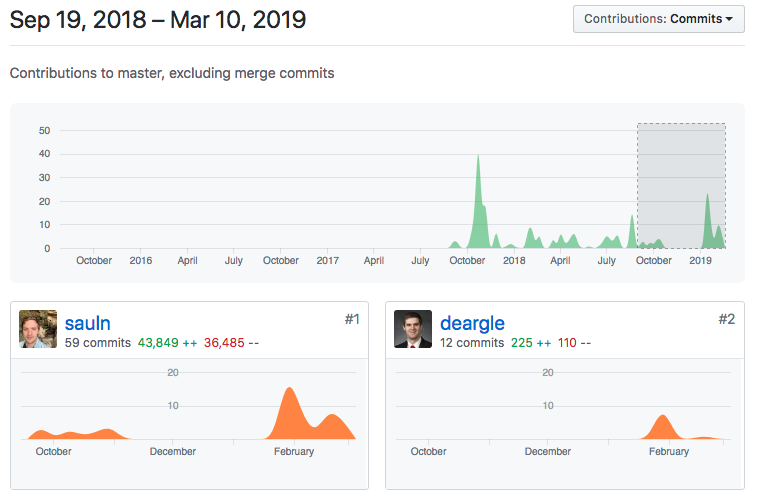
\includegraphics[width=0.8\textwidth]{images/keplermappergithubstats.png}
	\label{fig:keplermappergithubstats}
\end{figure} 
\begin{figure}[h!]
	\caption{KeplerMapper output example}
	\centering
	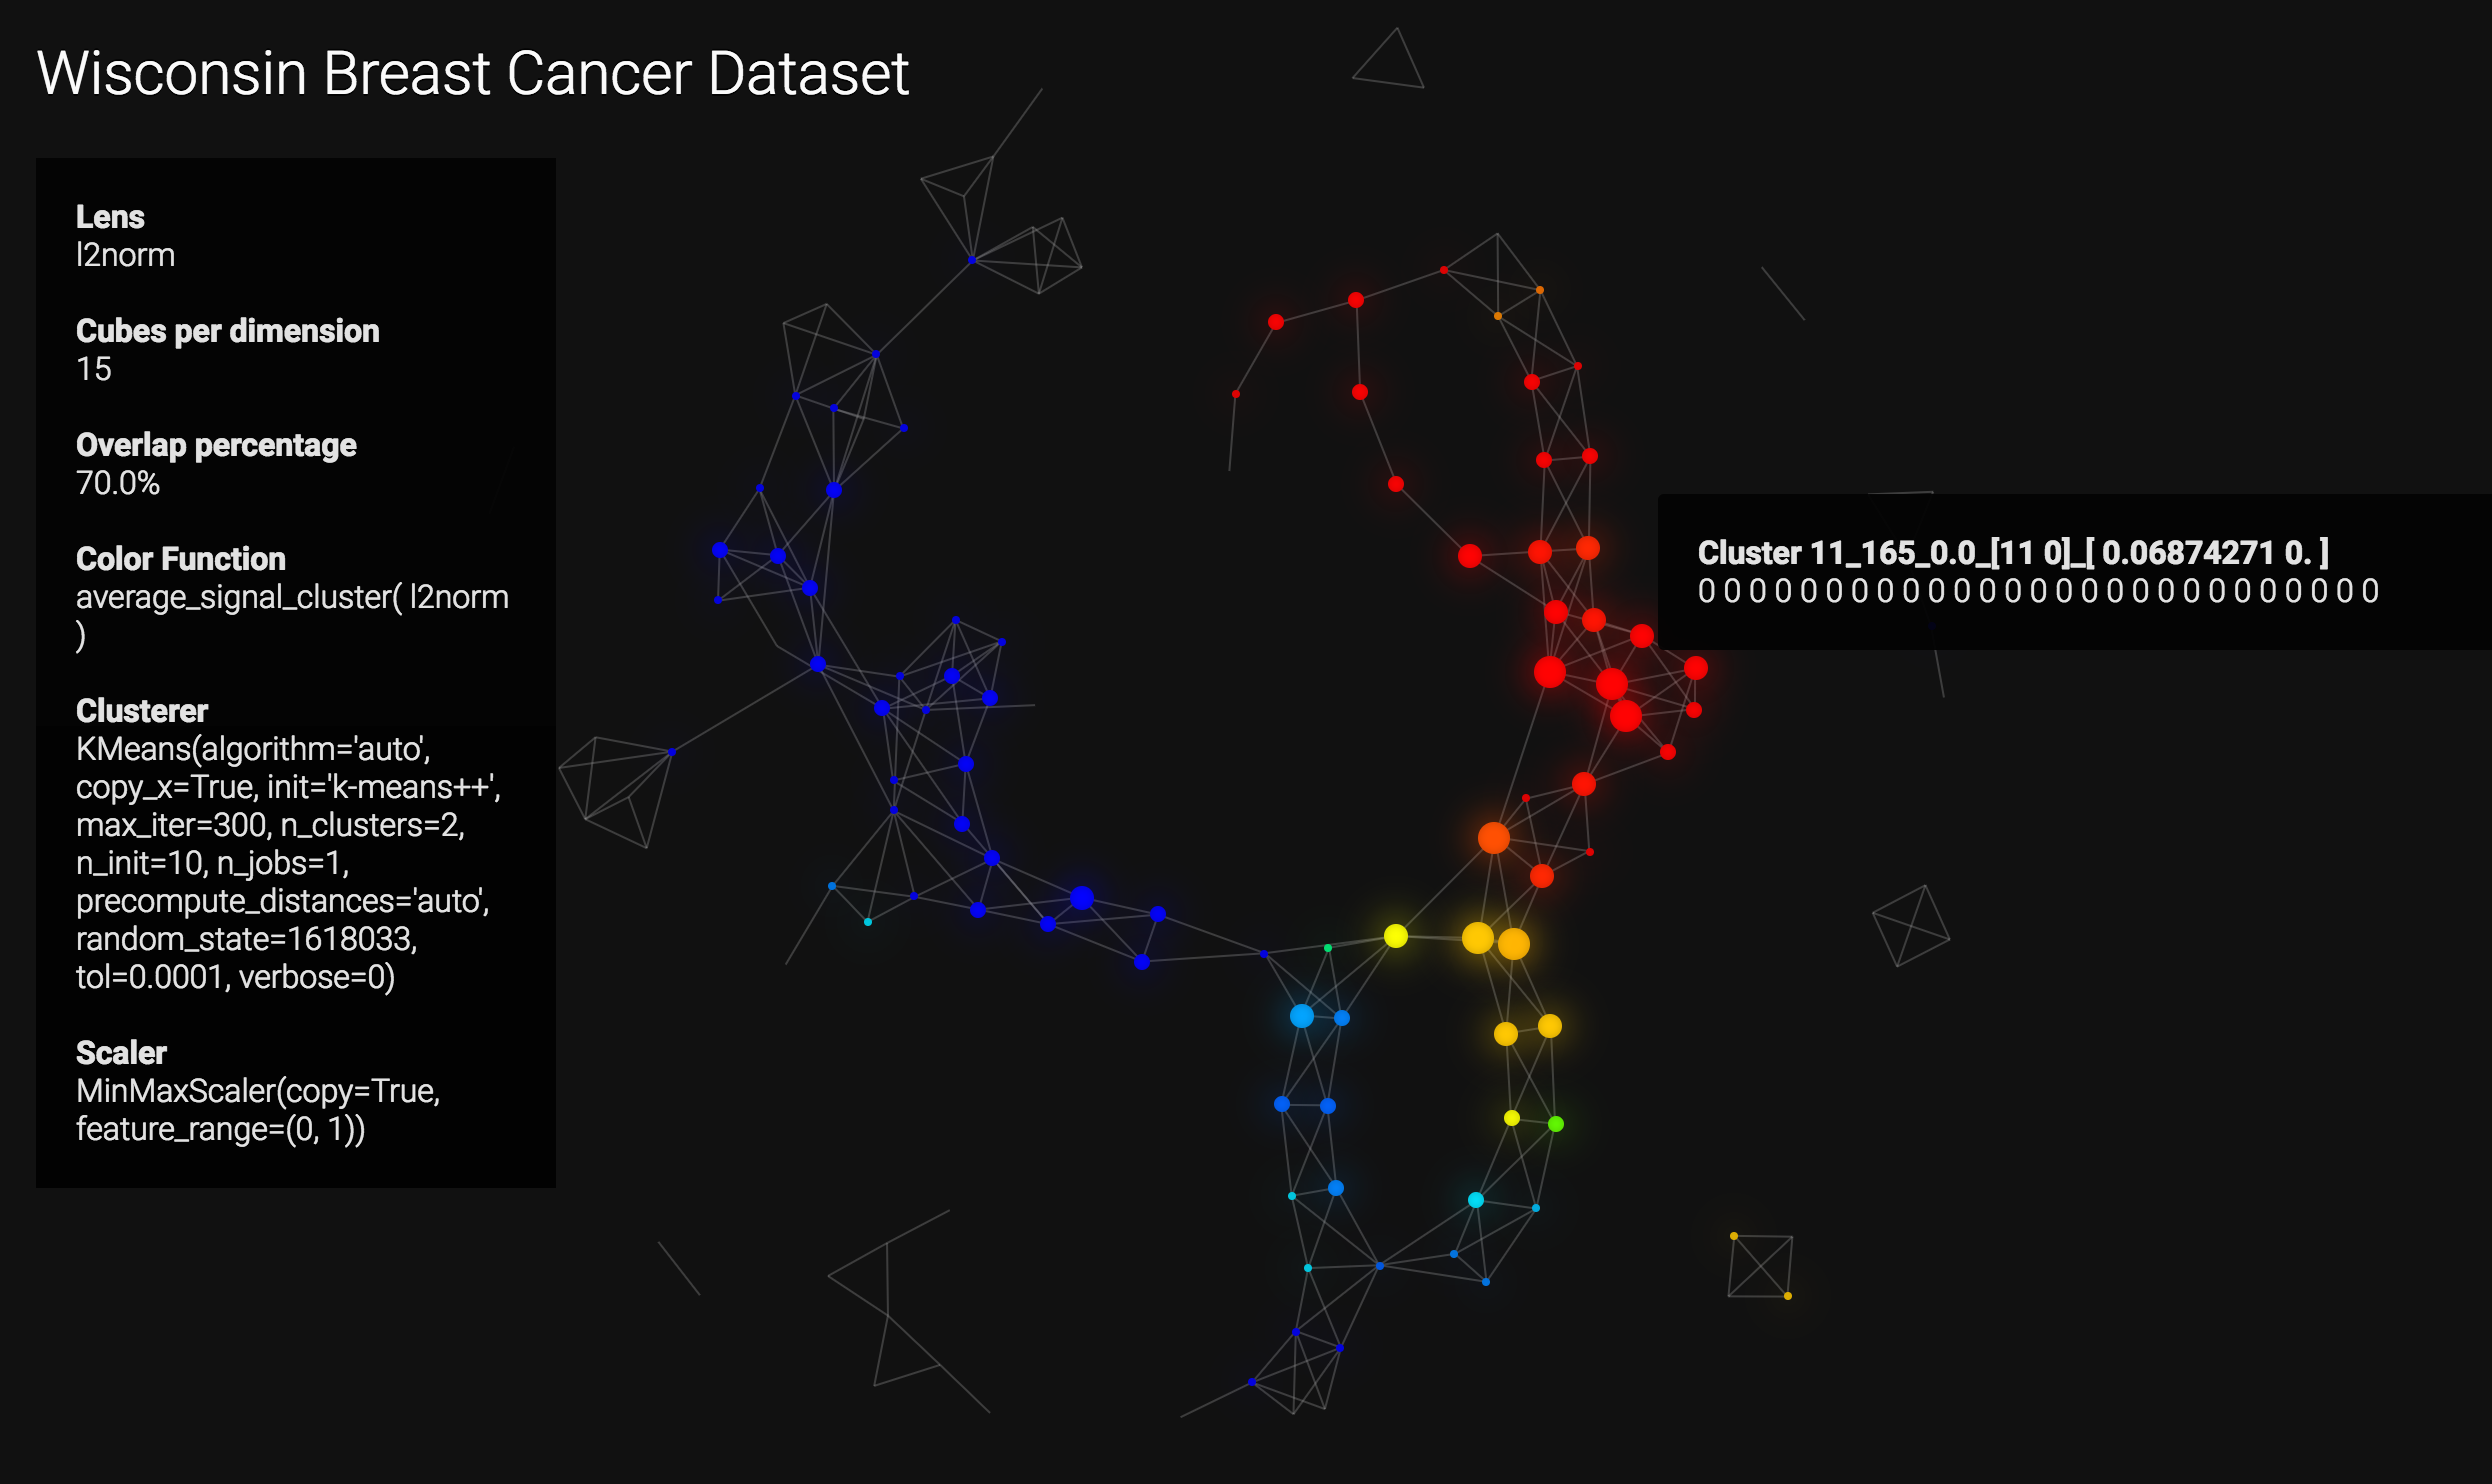
\includegraphics[width=0.8\textwidth]{images/keplermapper.png}
	\label{fig:keplermapperoutput}
\end{figure} 

\begin{figure}[h!]
\caption{Kepler Mapper Architecture (as in September 2018)}
\centering
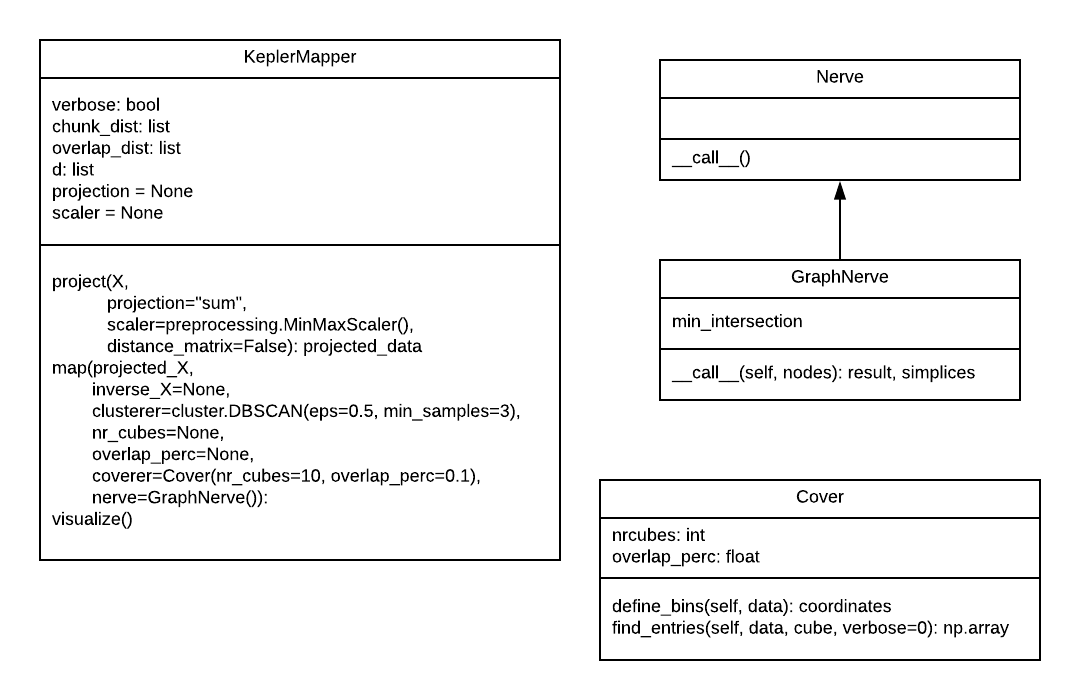
\includegraphics[width=0.8\textwidth]{images/KMapper.png}
\label{fig:keplermapper}
\end{figure}


\subsection{Python Mapper (PyMapper)}
Python Mapper is a Python package developed by Daniel M\"ullner as his PhD thesis. It comes with two companion packages written in C++: $cmappertools$ and $fastcluster$. Compared to Kepler Mapper, it is expected to be:
\begin{itemize}
	\item Comprehensive, thanks to the implementation of more filters, more covers.
	\item Performant, thanks to a custom C++ backend and thus compiled code and efficient multi threading.
	\item Easy to use, thanks to the graphical interface provided.
\end{itemize}

However, this package has the following cons:
\begin{itemize}
\item It is outdated and not maintained any more (Mapper: current release dated April 19, 2017. Cmappertools: current release dated March 2, 2016)
\item The code is not documented. A little documentation is provided for the use of the grapical interface, but there's no documentation about the native Python API.
\item No examples are provided with the code. However, it is possible to see the code generated by the GUI while playing around with simple datasets. An example of code generated by the GUI is given in Listing \ref{list:pymapper}
\item Code's architecture is in my opinion messy and poorly designed: there is no common interface of different filter classes and cover classes. There's a gigantic class $MapperOutput$ that is almost impossible to handle, given the many methods it offers. The code is organized as a mix of object oriented programming and functional programming making it really hard to understand how a modification will affect the whole system. The API of the package is not clear: in other words, it is not clear what is exposed to the user and what should be private.
\item C++ code is really hard to understand, since the original C-Python API is used instead of binding libraries such as PyBind11 (used in lmapper's companion package fastfilter). This makes the binding code really verbose and implementation-dependent.
\item It's really hard to install because of deprecated dependencies.
\item Some C++ implementations of clustering algorithms in $fastcluster$ are now obsolete, since they have been included in more recent releases of SciPy.
\end{itemize}

In figure \ref{fig:pymapper} a simplified UML class diagram of the core code of PyMapper is showed.
\begin{lstlisting}[language=Python, caption=PyMapper example automatically generated from the GUI, label=list:pymapper]
'''
    Python Mapper script
    Generated by the Python Mapper GUI
'''
import mapper
import numpy as np
import matplotlib.pyplot as plt

'''
    Step 1: Input
'''
import gzip
filename = '/Users/martinomilani/Documents/mapper/exampleshapes/cat-reference.csv.gz'
with gzip.open(filename, 'r') as inputfile:
    data = np.loadtxt(inputfile, delimiter=',', dtype=np.float)
# Preprocessing
point_labels = None
mask = None
Gauss_density = mapper.filters.Gauss_density
kNN_distance  = mapper.filters.kNN_distance
crop = mapper.crop
data, point_labels = mapper.mask_data(data, mask, point_labels)
'''
    Step 2: Metric
'''
intrinsic_metric = False
if intrinsic_metric:
    is_vector_data = data.ndim != 1
    if is_vector_data:
        metric = Euclidean
        if metric != 'Euclidean':
            raise ValueError('Not implemented')
    data = mapper.metric.intrinsic_metric(data, k=1, eps=1.0)
is_vector_data = data.ndim != 1
'''
    Step 3: Filter function
'''
if is_vector_data:
    metricpar = {'metric': 'euclidean'}
    f = mapper.filters.eccentricity(data,
        metricpar=metricpar,
        exponent=1.0)
else:
    f = mapper.filters.eccentricity(data,
        exponent=1.0)
# Filter transformation
mask = None
crop = mapper.crop
'''
    Step 4: Mapper parameters
'''
cover = mapper.cover.cube_cover_primitive(intervals=15, overlap=50.0)
cluster = mapper.single_linkage()
if not is_vector_data:
    metricpar = {}
mapper_output = mapper.mapper(data, f,
    cover=cover,
    cluster=cluster,
    point_labels=point_labels,
    cutoff=None,
    metricpar=metricpar)
cutoff = mapper.cutoff.first_gap(gap=0.1)
mapper_output.cutoff(cutoff, f, cover=cover, simple=False)
mapper_output.draw_scale_graph()
plt.savefig('scale_graph.pdf')
\end{lstlisting}

\begin{figure}[h]
\caption{PyMapper Architecture (simplified)}
\centering
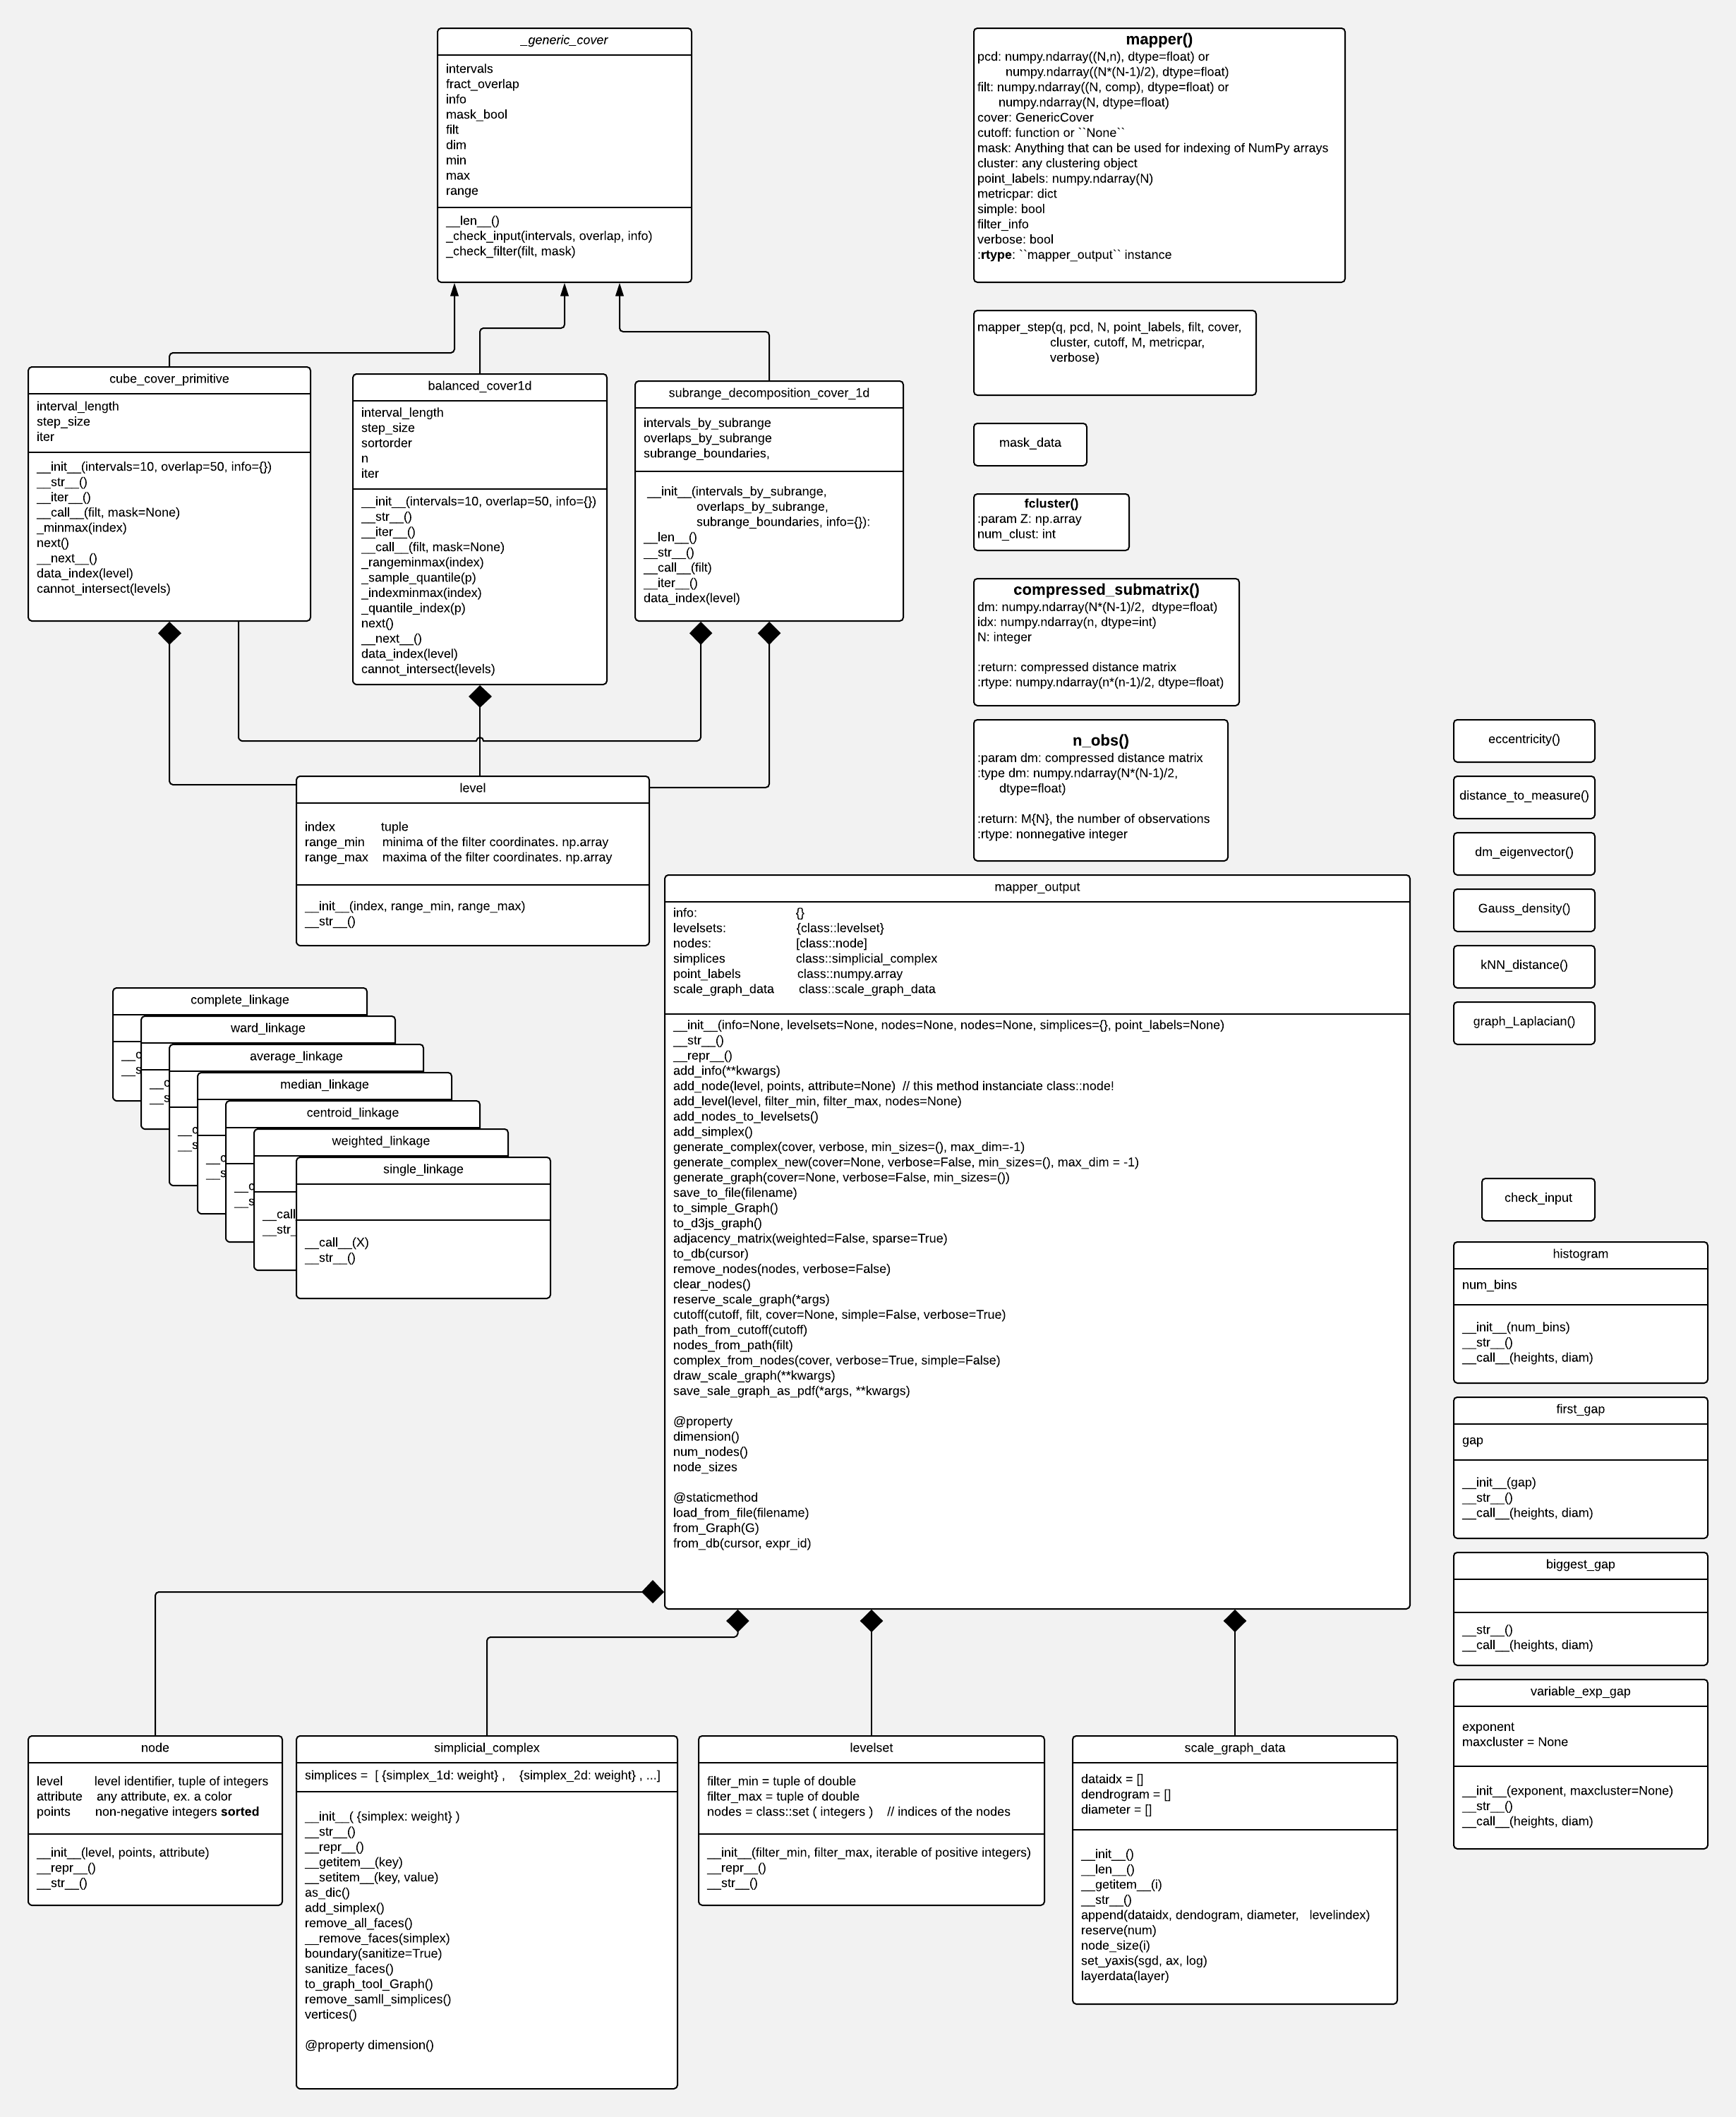
\includegraphics[width=0.8\textwidth]{images/pythonmapper.png}
\label{fig:pymapper}
\end{figure}

